\documentclass{beamer} % Use handout to get rid of repeated slides
\usetheme{AnnArbor}
\usecolortheme{default}
\usefonttheme{professionalfonts}
\usepackage{mathpazo}
\usepackage{listings}
\usepackage{xcolor}

% Define colors
\definecolor{myred}{RGB}{163,0,0}
\definecolor{ttcolor}{RGB}{0,0,1}%{RGB}{163,0,0}
\definecolor{mygray}{RGB}{248,249,250} 
\definecolor{mygreen1}{RGB}{0,96,0}
\definecolor{mygreen2}{RGB}{229,239,229}
\definecolor{aristotelgreen}{HTML}{008A44}
\definecolor{aristotelred}{HTML}{9E0101}
\definecolor{aristotelgrey}{HTML}{2E2E2E}
\definecolor{aristoteldarkred}{HTML}{500101}
\definecolor{aristotelorange}{HTML}{FF8C00}

\setbeamertemplate{theorem}[ams style]
\setbeamertemplate{theorems}[numbered]

\usepackage{etoolbox}
\usepackage{adjustbox}

\undef{\definition}
\theoremstyle{definition}
\newtheorem{definition}{\translate{Definition}}
\hypersetup{
	colorlinks=true,
	linkcolor=aristotelorange,   % color for normal internal links
	citecolor=aristotelgreen,   % color for citation links
	urlcolor=aristotelgreen      % color for external links
}

\setbeamercolor{palette primary}{bg=aristotelred, fg=white}
\setbeamercolor{palette secondary}{bg=aristoteldarkred, fg=white}
\setbeamercolor{palette tertiary}{bg=black, fg=white} 

\setbeamercolor{title}{fg=white, bg=aristotelred} % Title text color
\setbeamercolor{subtitle}{fg=white, bg=aristotelred} % Subtitle text color
\setbeamercolor{background canvas}{bg=aristotelgrey} % Background for content canvas
\setbeamercolor{normal text}{fg=white} % Normal text color
\setbeamercolor{titlegraphic}{bg=mygray} % Background color for title graphic area
\setbeamercolor{frametitle}{fg=white, bg=aristoteldarkred}

% Change color of numbered circles in the table of contents
\setbeamercolor{section number projected}{bg=white, fg=black}
\setbeamercolor{subsection number projected}{bg=aristotelred, fg=aristotelgrey}
\setbeamercolor{subsection number projected}{bg=aristotelorange, fg=white}

\setbeamercolor{block title}{fg=white,bg=mygreen1}
\setbeamercolor{block body}{fg=black,bg=mygreen2}


\lstdefinestyle{rstyle}%
{language=[LaTeX]TeX,
	basicstyle=\footnotesize\ttfamily,
	backgroundcolor = \color{mygray},
	commentstyle=\slshape\color{green!50!black},
	keywordstyle=\color{blue},
	identifierstyle=\color{blue},
	stringstyle=\color{orange},
	%escapechar=\#,
	rulecolor = \color{mygray}, 
	showstringspaces = false,
	showtabs = false,
	tabsize = 2,
	emphstyle=\color{red},
	frame = single} 

\begin{document}
	\title[HW: IVs]{Homework}
	\subtitle[subtitle?]{Order Logit\\
		Survey of Outlook of the Economy}
	\author[Riste Petrov]{Riste Petrov \\ \href{mailto:riste@uni-sofia.bg}{riste@uni-sofia.bg}}
	\institute[AEEM - FEBA]{AEEM - FEBA - Sofia University St. Kliment Ohridski - coh. 2026/27}
	\titlegraphic{\includegraphics[scale=0.5]{/home/anonymous/Documents/Mega Sync/ЦЕЛ/Master/1Courses/SU ENG White horizontal.pdf}}
	\date{\today}
	
	\begin{frame}[fragile]
		\titlepage
	\end{frame}
	
	\begin{frame}[fragile]
		\frametitle{Contents}
		\tableofcontents[]
	\end{frame}
	
	\section{Why predicting PPP?}
	\begin{frame}[fragile]
		\frametitle{Why predicting PPP?}
		\begin{center}
		\begin{tabular}{|c|c|c|c|c|c|}
			\hline
			COICOP & MKD & 2 mean salary & Ratio & Base & Chain \\
			\hline
			2020M01 & 31,169.67 &  &  &  &  \\
			2021M01 & 32,101.33 &  &  &  &  \\
			2022M01 & 32,084.67 &  &  &  &  \\
			2023M01 & 32,084.67 &  &  &  &  \\
			2024M01 & 35,099.33 &  &  &  &  \\
			\hline
			\_\_\_\_\_ &  &  &  &  &  \\
			\hline
		\end{tabular}
		\vspace{1em}
		
		\begin{tabular}{|c|c|c|c|c|c|}
			\hline
			SSM & MKD  & 2 mean salary & Ratio & Base & Chain \\
			\hline
			2020M01 & 32,791.00 &  &  &  &  \\
			2021M01 & 33,650.00 &  &  &  &  \\
			2022M01 & 35,811.00 &  &  &  &  \\
			2023M01 & 50,799.00 &  &  &  &  \\
			2024M01 & 57,163.00 &  &  &  &  \\
			\hline
			\_\_\_\_\_ &  &  &  &  &  \\
			\hline
		\end{tabular}
		\end{center}
	\end{frame}
	
	
	
	\begin{frame}[fragile]
		\frametitle{Correlation Matrix}  
		\small
		\begin{center}
		\begin{adjustbox}{max height=\textheight-2\baselineskip}
			  
		\begin{tabular}{l c}
		\hline  
			          & \textbf{B7\_PPP\_NOW} \\ 
		\hline
		B6\_WAGE\_1M          & $ 0.29$              \\     
		B5\_WAGE\_NOW         & $ 0.39$              \\
		B14\_2\_LOWERWAGE     & -$0.27$             \\
		B14\_1\_WORK          & -$0.15$             \\      
		\hline     
		B3\_ID\_NOW           & $ 0.49$              \\      
		B4\_ID\_1M            & $ 0.33$              \\
		\hline   
		B1\_BG\_NOW           & $ 0.27$              \\         
		B2\_3\_BG\_12M        & $ 0.13$              \\
		\hline
		B14\_9\_NOBIGSHOP     & -$0.29$             \\     
		B14\_8\_SPENDSAVE     & -$0.20$             \\      
		B14\_6\_DOSAVE        & $ 0.20$              \\      		      
		\hline
		CITY                  & $ 0.09$             \\      
		EDU                   & $ 0.06$              \\      
		WAGE                  & -$0.29$             \\          
		\hline
		\end{tabular}  \end{adjustbox}  \end{center}
	\end{frame}
	
	\begin{frame}[fragile] 
		\frametitle{Model} 
		\begin{center}
			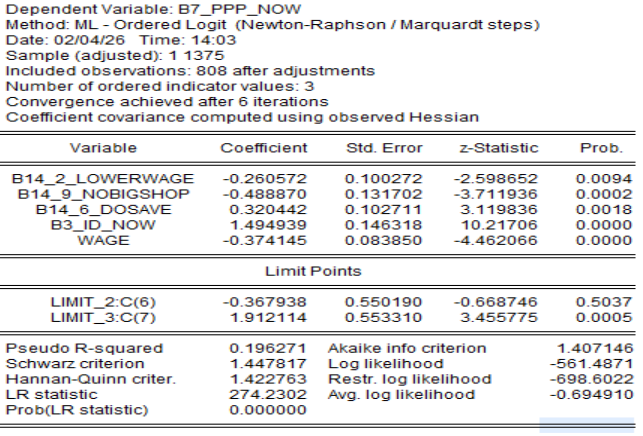
\includegraphics[height=0.8\textheight]{model.png}	
		\end{center}
	
	
	\end{frame}
	
	\section{Q\&A}
	\begin{frame}[fragile]
		\frametitle{Ending remarks}
		\begin{center}
			I am delighted for your attention.\\
			\vspace{1em}
			Q \& A?
		\end{center}
	\end{frame}
	
\end{document}